% r3d2.tex

% Final project writeup.

% This file is part of R3D2.

% R3D2 is free software: you can redistribute it and/or modify
% it under the terms of the GNU General Public License as published by
% the Free Software Foundation, either version 3 of the License, or
% (at your option) any later version.

% R3D2 is distributed in the hope that it will be useful,
% but WITHOUT ANY WARRANTY; without even the implied warranty of
% MERCHANTABILITY or FITNESS FOR A PARTICULAR PURPOSE. See the
% GNU General Public License for more details.

% You should have received a copy of the GNU General Public License
% along with this program. If not, see <https://www.gnu.org/licenses/>.

\documentclass{article}

\usepackage{caption}
\usepackage[american, siunitx]{circuitikz}
\usepackage{geometry}[margin=1in]
\usepackage{siunitx}
\usepackage{subcaption}
\usepackage{tikz}
\usepackage{underscore}

\usetikzlibrary{automata}

\ctikzset{monopoles/vcc/arrow=Stealth}

\title{R3D2: An ESP32-powered object-avoiding robot}
\author{Owen Niles}
\date{10 May 2020}

\begin{document}

\maketitle

\begin{abstract}

  R3D2 is an autonomous robot that can navigate through indoor spaces without
  bumping into obstacles such as walls and large household objects similarly to
  the way in which a Rumba or similar product does the same. The code running
  on R3D2's microcontroller, the ESP32, implements a finite state machine,
  which helps R3D2 understand and make decisions about its surroundings. The
  code allows the microcontroller to communicate with various peripherals,
  which provide inputs to and accept outputs from the finite state machine.

\end{abstract}

\section{Introduction} \label{sec:intro}

R3D2's brain is the ESP32 microcontroller, which I already had lying around my
house. I chose this microcontroller because I liked the relatively low-level
programming interface that it provided and because the chip comes with WiFi and
Bluetooth hardware. I thought it would be nice to be able to add WiFi and
Bluetooth connectivity to my project if I had extra time, which I did not have.

The components are powered by two separate power sources; a \SI{5}{\volt}
portable phone charger powers the microcontroller, while a \SI{6}{\volt} pack
of 4 AA batteries provides a higher bias for those components that require more
than the \SI{3.3}{\volt} that the microcontroller is capable of outputting.

R3D2 achieves object-avoidance by reading data from two ultrasonic distance
sensors, mounted 135$^\circ$ apart in its head, which itself is allowed
135$^\circ$ of rotation. When R3D2's head rotates, the distance sensors give
the robot as it were 270$^\circ$ of vision.

Based on data supplied by the distance sensors, R3D2 makes decisions, which
are communicated to two motors that drive the wheels, about how to move. If
R3D2 doesn't detect any obstacles closer than some threshold distance in front
of itself, it moves forward and continues to measure the ditance to the closest
obstacle directly in front of it. However, if there is an obstacle immediately
in front of R3D2, it scans its surroundings for an alternative path, choosing
the one along which the next obstacle is furthest away.

\section{Design}

\subsection{Theoretical design} \label{sec:fsm}

We can model R3D2's decision-making process as a finite state machine
$T = (Q,\Sigma,\Gamma,I,F,\delta)$. $Q = q_0q_1$ is the set of $T$'s states,
where $q_0$ represents the state of scanning for an alternative path and $q_1$
represents the state of pinging for objects immediately in front of itself.
$\Sigma = a_0a_1a_2a_3$ is the input alphabet, where $a_0$ represents the
absence of any nearby obstacles, $a_1$ represents the presence of an object
immediately in front of the robot, and $a_2,a_3$ represent the presence of the
nearest obstacle to its left and right respectively. $\Gamma = b_0b_1b_2b_3$ isthe output alphabet, where $b_0$ represents the microcontroller telling the
drive motors to stop, $b_1$ represents the microcontroller telling them to move
the robot forward, and $b_2,b_3$ represent the microcontroller telling them to
turn the robot left and right respectively. Finally, $I = q_0$ and
$F = \emptyset$ are the sets of initial and final states and $\delta$ is the
transition function as it is described at the end of section \ref{sec:intro}.

Figure \ref{fig:fsm} shows a visualization of $(Q,\delta)$.

\begin{figure}[h]
  \centering
  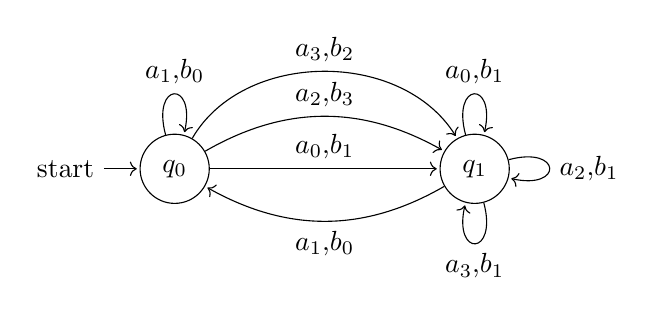
\begin{tikzpicture}[shorten >=1pt, node distance=1.5in, auto]
    \node[state, initial](q0){$q_0$};
    \node[state](q1)[right of=q0]{$q_1$};
    \path[->] (q0) edge node{$a_0$,$b_1$} (q1)
    (q0) edge[loop above] node{$a_1$,$b_0$} (q0)
    (q0) edge[bend left] node{$a_2$,$b_3$} (q1)
    (q0) edge[bend left=60] node{$a_3$,$b_2$} (q1)
    (q1) edge[loop above] node{$a_0$,$b_1$} (q1)
    (q1) edge[bend left] node{$a_1$,$b_0$} (q0)
    (q1) edge[loop right] node{$a_2$,$b_1$} (q1)
    (q1) edge[loop below] node{$a_3$,$b_1$} (q1);
  \end{tikzpicture}
  \caption{A visualization of the finite state machine $T$ (rather informally)
    formalized in section \ref{sec:fsm} that helps R3D2 understand and make
    decisions about its surroundings.}
  \label{fig:fsm}
\end{figure}

\subsection{Circuit design}

Unfortunately, R3D2's circuitry is not terribly complex. I implemented two
identical voltage dividers and a power kill switch, but most of the components
are connected directly using wires without the need for complex circuitry. the voltage dividers were useful because they halved the voltage of one particular
output signal and the kill switch allowed me to quickly connect and disconnect
power, which facilitated rapid testing.

Figures \ref{fig:div} and \ref{fig:switch} contain diagrams of the circuitry
that I implemented on my own. Figure \ref{fig:schema} contains the remainder
of the full circuit schematic.

\subsubsection{Voltage divider}

In order to allow the distance sensors to communicate safely with the
microcontroller, I had to step the sensors' output voltage down from
\SI{6}{\volt} to roughly \SI{3.3}{\volt}, which is the maximum voltage for
which the microcontroller's pins are rated.

To achieve this step down in voltage, I implemented two voltage dividers using
four \SI{330}{\ohm} resistors as shown in figure \ref{fig:div}

\begin{figure}
  \begin{center}
    \begin{subfigure}{0.4\textwidth}
      \centering
      \begin{circuitikz}
        \draw (0,0) coordinate(echo) to[R=330<\ohm>, a=$R_0$, *-*] ++(0,-2)
        coordinate(tmp) to[R=330<\ohm>, a=$R_1$] ++(0,-2) node[ground]{};
        \draw (tmp) -- ++(2,0) node[vcc, rotate=-90](pin){};
        \draw (echo) node[anchor=south]{\texttt{DIST0_ECHO_PIN}};
        \draw (pin) node[anchor=south]{\texttt{GPIO\_NUM\_36}};
      \end{circuitikz}
      \caption{The voltage divider used to step the distance sensor
        \texttt{DIST0}'s output voltage down from roughly \SI{6}{\volt} to
        roughly \SI{3}{\volt}.}
    \end{subfigure}
    \hspace{0.1\textwidth}
    \begin{subfigure}{0.4\textwidth}
      \centering
      \begin{circuitikz}
        \draw (0,0) coordinate(echo) to[R=330<\ohm>, a=$R_2$, *-*] ++(0,-2)
        coordinate(tmp) to[R=330<\ohm>, a=$R_3$] ++(0,-2) node[ground]{};
        \draw (tmp) -- ++(2,0) node[vcc, rotate=-90](pin){};
        \draw (echo) node[anchor=south]{\texttt{DIST1_ECHO_PIN}};
        \draw (pin) node[anchor=south]{\texttt{GPIO\_NUM\_39}};
      \end{circuitikz}
      \caption{The voltage divider used to step the distance sensor
        \texttt{DIST1}'s output voltage down from roughly \SI{6}{\volt} to
        roughly \SI{3}{\volt}.}
    \end{subfigure}
    \caption{Voltage dividers used to halve the voltage of the distance
      sensors' output signal.}
    \label{fig:div}
  \end{center}
\end{figure}

\subsubsection{Power kill switch}

Since I was using two different power sources and I constantly found myself
disconnecting and reconnecting them, I decided that I wanted a convenient way
to accomplish this task quickly.

The circuit that I implemented was neither complicated nor critical to R3D2's
operation, but it was quite useful. I have provided a schematic diagram of it
in figure \ref{fig:switch}.

\begin{figure}
  \centering
  \begin{circuitikz}
    \draw (0,0) node[cute spdt mid arrow, rotate=-90](switch){};
    \draw (switch.in) node[anchor=south east]{Bias kill switch};
    \draw (switch.in) -- ++(2,0) coordinate(branch) to[short, -o] ++(2,0)
    node[anchor=west]{$v_{cc}$};
    \draw (switch.out 2) -- ++(0,-3) node[ground](gnd){};
    \draw (switch.out 1) to[battery1=6<\volt>] (switch.out 1 |- gnd)
    node[ground]{};
    \draw (branch) to[empty led, l2={Green power indicator} and {\ }, *-]
    ++(0,-2) coordinate(mid) to[R=330<\ohm>, a=$R_4$] (branch |- gnd)
    node[ground]{};
  \end{circuitikz}
  \caption{A simple kill switch and power indicator LED that I implemented so
    that I could easily disconnect the \SI{6}{\volt} bias.}
  \label{fig:switch}
\end{figure}

\begin{figure}[h]
  \centering
  \resizebox{!}{\textheight}{\begin{circuitikz}
    % Draw ESP32
    \draw (-2,0) node[dipchip, num pins=38, hide numbers, no topmark,
      external pins width=0](esp32) {\texttt{ESP32}};
    \draw (esp32.bpin 3) to[short, -*, a=\texttt{GPIO_NUM_36}, font=\small]
    ++(-3,0);
    \draw (esp32.bpin 4) to[short, -*, a=\texttt{GPIO_NUM_39}, font=\small]
    ++(-3,0);
    \draw (esp32.bpin 9) to[short, -*, a=\texttt{GPIO_NUM_25}, font=\small]
    ++(-3,0);
    \draw (esp32.bpin 10) to[short, -*, a=\texttt{GPIO_NUM_26}, font=\small]
    ++(-3,0);
    \draw (esp32.bpin 14) -- ++(-1,0) coordinate(tmp) -- (tmp |- esp32.south)
    node[ground]{};
    \draw (esp32.bpin 26) to[short, -*, l=\texttt{GPIO_NUM_4}, font=\small]
    ++(3,0);
    \draw (esp32.bpin 27) to[short, -*, l=\texttt{GPIO_NUM_16}, font=\small]
    ++(3,0);
    \draw (esp32.bpin 28) to[short, -*, l=\texttt{GPIO_NUM_17}, font=\small]
    ++(3,0);
    \draw (esp32.bpin 29) to[short, -*, l=\texttt{GPIO_NUM_5}, font=\small]
    ++(3,0);
    \draw (esp32.bpin 30) to[short, -*, l=\texttt{GPIO_NUM_18}, font=\small]
    ++(3,0);
    \draw (esp32.bpin 31) to[short, -*, l=\texttt{GPIO_NUM_19}, font=\small]
    ++(3,0);
    \draw (esp32.bpin 32) -- ++(4,0) coordinate(tmp);
    \draw (esp32.bpin 33) to[short, -*, l=\texttt{GPIO_NUM_21}, font=\small]
    ++(3,0);
    \draw (esp32.bpin 36) to[short, -*, l=\texttt{GPIO_NUM_22}, font=\small]
    ++(3,0);
    \draw (esp32.bpin 37) to[short, -*, l=\texttt{GPIO_NUM_23}, font=\small]
    ++(3,0);
    \draw (esp32.bpin 38) -- (tmp |- esp32.bpin 38) -- (tmp |- esp32.south)
    node[ground]{};

    % Draw distance sensor 0
    \draw (6,4) node[dipchip, num pins=12, hide numbers, no topmark,
      external pins width=0, rotate=90](dist0){
      \rotatebox{-90}{\texttt{HC-SR04 (DIST0)}}};
    \draw (dist0.bpin 2) -- ++(0,-1.5) coordinate(tmp) to[short, -*,
      font=\small] ++(0,-1.5);
    \draw (tmp) node[anchor=south, rotate=90, font=\small]{
      \texttt{DIST0_VCC_PIN}};
    \draw (dist0.bpin 3) to[short, -*] ++(0,-3);
    \draw (dist0.bpin 3 |- tmp) node[anchor=south, rotate=90, font=\small]{
      \texttt{DIST0_TRIG_PIN}};
    \draw (dist0.bpin 4) to[short, -*] ++(0,-3);
    \draw (dist0.bpin 4 |- tmp) node[anchor=south, rotate=90, font=\small]{
      \texttt{DIST0_ECHO_PIN}};
    \draw (dist0.bpin 5) node[ground]{};

    % Draw distance sensor 1
    \draw (6,-2) node[dipchip, num pins=12, hide numbers, no topmark,
      external pins width=0, rotate=90](dist1){
      \rotatebox{-90}{\texttt{HC-SR04 (DIST1)}}};
    \draw (dist1.bpin 2) -- ++(0,-1.5) coordinate(tmp) to[short, -*]
    ++(0,-1.5);
    \draw (dist1.bpin 3) to[short, -*] ++(0,-3);
    \draw (dist1.bpin 4) to[short, -*] ++(0,-3);
    \draw (dist1.bpin 5) node[ground]{};
    \draw (tmp) node[anchor=south, rotate=90, font=\small]{
      \texttt{DIST1_VCC_PIN}};
    \draw (dist1.bpin 3 |- tmp) node[anchor=south, rotate=90, font=\small]{
      \texttt{DIST1_TRIG_PIN}};
    \draw (dist1.bpin 4 |- tmp) node[anchor=south, rotate=90, font=\small]{
      \texttt{DIST1_ECHO_PIN}};
    
    % Draw servo
    \draw (10,0) node[dipchip, num pins=6, hide numbers, no topmark,
      external pins width=0, rotate=90](servo){};
    \draw (servo.bpin 1) -- ++(0,-1.5) coordinate(mid) to[short, -*,
      font=\small] ++(0,-1.5) coordinate(bottom);
    \draw (servo.bpin 2) to[short, -*] (servo.bpin 2 |- bottom);
    \draw (servo.bpin 3) node[ground]{};
    \draw (servo.bpin 5) node[anchor=south]{\texttt{SO5NF STD (SERVO)}};
    \draw (mid) node[anchor=south, rotate=90, font=\small]{
      \texttt{SERVO_VCC_PIN}};
    \draw (servo.bpin 2 |- mid) node[anchor=south, rotate=90, font=\small]{
      \texttt{SERVO_PULSE_PIN}};
    
    \ctikzset{multipoles/dipchip/width=3}

    % Draw motor driver
    \draw (5,-9) node[dipchip, num pins=16, hide numbers, no topmark,
      external pins width=0](driver){\texttt{TB6612FNG (DRIVER)}};
    \draw (driver.bpin 1) to[short, -*, a=\texttt{DRIVER_VM_PIN},
    font=\small] ++(-3,0);
    \draw (driver.bpin 2) to[short, -*, a=\texttt{DRIVER_VCC_PIN}, font=\small]
    ++(-3,0);
    \draw (driver.bpin 8) -- ++(-1,0) coordinate(tmp);
    \draw (tmp |- driver.bpin 4) node[jump crossing](a1){};
    \draw (tmp |- driver.bpin 5) node[jump crossing](a2){};
    \draw (tmp |- driver.bpin 6) node[jump crossing](b2){};
    \draw (tmp |- driver.bpin 7) node[jump crossing](b1){};
    \draw (driver.bpin 3) -- (tmp |- driver.bpin 3) -- (a1.north);
    \draw (a1.south) -- (a2.north);
    \draw (a2.south) -- (b2.north);
    \draw (b2.south) -- (b1.north);
    \draw (b1.south) -- (tmp |- driver.south) node[ground]{};
    \draw (driver.bpin 4) -- (a1.east);
    \draw (driver.bpin 5) -- (a2.east);
    \draw (driver.bpin 6) -- (b2.east);
    \draw (driver.bpin 7) -- (b1.east);
    \draw (driver.bpin 9) -- ++(1,0) coordinate(tmp) -- (tmp |- driver.south)
    node[ground]{};
    \draw (driver.bpin 10) to[short, -*, l=\texttt{DRIVER_PWMB_PIN},
    font=\small] ++(3,0);
    \draw (driver.bpin 11) to[short, -*, l=\texttt{DRIVER_B2_PIN}, font=\small]
    ++(3,0);
    \draw (driver.bpin 12) to[short, -*, l=\texttt{DRIVER_B1_PIN}, font=\small]
    ++(3,0);
    \draw (driver.bpin 13) to[short, -*, l=\texttt{DRIVER_STBY_PIN},
      font=\small] ++(3,0);
    \draw (driver.bpin 14) to[short, -*, l=\texttt{DRIVER_A1_PIN}, font=\small]
    ++(3,0);
    \draw (driver.bpin 15) to[short, -*, l=\texttt{DRIVER_A2_PIN}, font=\small]
    ++(3,0);
    \draw (driver.bpin 16) to[short, -*, l=\texttt{DRIVER_PWMA_PIN},
      font=\small] ++(3,0);

    % Draw motor A
    \draw (-3,-9) node[elmech](a){\texttt{A}};
    \draw (0,-11) node[elmech](b){\texttt{B}};
    \draw (a1.west) -- ++(-3,0) -- ++(0,1) coordinate(tmp) -- (a |- tmp)
    -- (a.top);
    \draw (a2.west) -- ++(-3,0) -- ++(0,-1) coordinate(tmp) -- (a |- tmp)
    -- (a.bottom);
    \draw (b2.west) -- (b |- b2.west) -- (b.top);
    \draw (b1.west) -- ++(-1,0) -- ++(0,-2) coordinate(tmp) -- (b |- tmp)
    -- (b.bottom);

    % GPIO_NUM_4 -> DRIVER_B2_PIN
    \draw (-5,-14) coordinate(left) to[short, *-] ++(6,0)
    node[vcc,rotate=-90](right){};
    \draw (left) node[anchor=south, font=\small]{\texttt{GPIO_NUM_4}};
    \draw (right) node[anchor=south, font=\small]{\texttt{DRIVER_B2_PIN}};
    
    % GPIO_NUM_5 -> DRIVER_A1_PIN
    \draw (-5,-15) coordinate(left) to[short, *-] ++(6,0)
    node[vcc,rotate=-90](right){};
    \draw (left) node[anchor=south, font=\small]{\texttt{GPIO_NUM_5}};
    \draw (right) node[anchor=south, font=\small]{\texttt{DRIVER_A1_PIN}};
    
    % GPIO_NUM_16 -> DRIVER_B1_PIN
    \draw (-5,-16) coordinate(left) to[short, *-] ++(6,0)
    node[vcc,rotate=-90](right){};
    \draw (left) node[anchor=south, font=\small]{\texttt{GPIO_NUM_16}};
    \draw (right) node[anchor=south, font=\small]{\texttt{DRIVER_B1_PIN}};
    
    % GPIO_NUM_17 -> DRIVER_A2_PIN
    \draw (-5,-17) coordinate(left) to[short, *-] ++(6,0)
    node[vcc,rotate=-90](right){};
    \draw (left) node[anchor=south, font=\small]{\texttt{GPIO_NUM_17}};
    \draw (right) node[anchor=south, font=\small]{\texttt{DRIVER_A2_PIN}};
    
    % GPIO_NUM_18 -> DIST1_TRIG_PIN
    \draw (-5,-18) coordinate(left) to[short, *-] ++(6,0)
    node[vcc,rotate=-90](right){};
    \draw (left) node[anchor=south, font=\small]{\texttt{GPIO_NUM_18}};
    \draw (right) node[anchor=south, font=\small]{\texttt{DIST1_TRIG_PIN}};
    
    % GPIO_NUM_19 -> DIST0_TRIG_PIN
    \draw (-5,-19) coordinate(left) to[short, *-] ++(6,0)
    node[vcc,rotate=-90](right){};
    \draw (left) node[anchor=south, font=\small]{\texttt{GPIO_NUM_19}};
    \draw (right) node[anchor=south, font=\small]{\texttt{DIST0_TRIG_PIN}};
    
    % GPIO_NUM_21 -> DRIVER_PWMB_PIN
    \draw (5,-14) coordinate(left) to[short, *-] ++(6,0)
    node[vcc,rotate=-90](right){};
    \draw (left) node[anchor=south, font=\small]{\texttt{GPIO_NUM_21}};
    \draw (right) node[anchor=south, font=\small]{\texttt{DRIVER_PWMB_PIN}};
    
    % GPIO_NUM_22 -> DRIVER_PWMA_PIN
    \draw (5,-15) coordinate(left) to[short, *-] ++(6,0)
    node[vcc,rotate=-90](right){};
    \draw (left) node[anchor=south, font=\small]{\texttt{GPIO_NUM_22}};
    \draw (right) node[anchor=south, font=\small]{\texttt{DRIVER_PWMA_PIN}};
    
    % GPIO_NUM_23 -> SERVO_PULSE_PIN
    \draw (5,-16) coordinate(left) to[short, *-] ++(6,0)
    node[vcc,rotate=-90](right){};
    \draw (left) node[anchor=south, font=\small]{\texttt{GPIO_NUM_23}};
    \draw (right) node[anchor=south, font=\small]{\texttt{SERVO_PULSE_PIN}};

    % 3.3 V source
    \draw (5,-17) coordinate(left0) to[short, *-] ++(2,0) -- ++(0,-0.5)
    coordinate(left) -- ++(2,0) coordinate(right) -- ++(0,0.5) -- ++(2,0)
    node[vcc, rotate=-90](right0){};
    \draw (5,-18) coordinate(left1) to[short, *-] (left |- left1) -- (left);
    \draw (right) -- ++(0,-0.5) coordinate(tmp) -- (right0 |- tmp)
    node[vcc, rotate=-90](right1){};
    \draw (left0) node[anchor=south, font=\small]{\texttt{GPIO_NUM_25}};
    \draw (left1) node[anchor=south, font=\small]{\texttt{GPIO_NUM_26}};
    \draw (right0) node[anchor=south, font=\small]{\texttt{DRIVER_VCC_PIN}};
    \draw (right1) node[anchor=south, font=\small]{\texttt{DRIVER_STBY_PIN}};

    % Draw connection to batteries
    \draw (0,-20.5) coordinate(left) to[short, o-] ++(4,0) coordinate(right)
    -- ++(0,0.5) coordinate(tmp) -- ++(2,0) node[vcc, rotate=-90](right1){};
    \draw (tmp) -- ++(0,1) coordinate(tmp) -- (right1 |- tmp)
    node[vcc, rotate=-90](right0){};
    \draw (right) -- ++(0,-0.5) coordinate(tmp) -- (right1 |- tmp)
    node[vcc, rotate=-90](right2){};
    \draw (tmp) -- ++(0,-1) coordinate(tmp) -- (right1 |- tmp)
    node[vcc, rotate=-90](right3){};
    \draw (left) node[anchor=south]{$v_{cc}$};
    \draw (right0) node[anchor=south, font=\small]{\texttt{SERVO_VCC_PIN}};
    \draw (right1) node[anchor=south, font=\small]{\texttt{DRIVER_VM_PIN}};
    \draw (right2) node[anchor=south, font=\small]{\texttt{DIST0_VCC_PIN}};
    \draw (right3) node[anchor=south, font=\small]{\texttt{DIST1_VCC_PIN}};
  \end{circuitikz}}
  \caption{R3D2's wiring schematic.}
  \label{fig:schema}
\end{figure}

\end{document}
